\documentclass[border=4pt]{standalone}
\usepackage{amsmath,amssymb,bm,mathtools}
\usepackage{tikz}
\usetikzlibrary{positioning,calc}
\usepackage{xcolor}
\definecolor{blue}{HTML}{1F618D}\definecolor{red}{HTML}{B03A2E}\definecolor{gray}{HTML}{7F7F7F}
\definecolor{ink}{HTML}{111111}
\begin{document}
\color{ink}
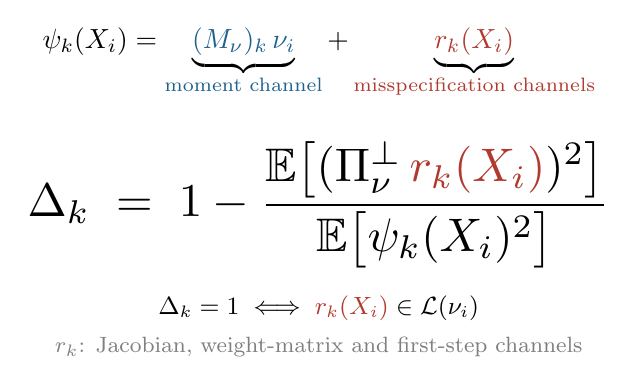
\begin{tikzpicture}[every node/.style={inner sep=0pt,outer sep=0pt}]
% LINE 1: decomposition of the influence function (Corollary 1, p.12 printed)
\node (l1) {$\displaystyle \psi_k(X_i)=\underbrace{\textcolor{blue}{(M_\nu)_k\,\nu_i}}_{\textcolor{blue}{\text{moment channel}}}+\underbrace{\textcolor{red}{r_k(X_i)}}_{\textcolor{red}{\text{misspecification channels}}}$};
% LINE 2: informativeness as one minus the out-of-span share (dominant element)
\node[below=16pt of l1, scale=1.7] (l2) {$\displaystyle \Delta_k \;=\; 1-\frac{\mathbb{E}\big[(\Pi_\nu^{\perp}\,\textcolor{red}{r_k(X_i)})^2\big]}{\mathbb{E}\big[\psi_k(X_i)^2\big]}$};
% LINE 3: the iff characterisation
\node[below=10pt of l2, font=\small] (l3) {$\Delta_k=1 \iff \textcolor{red}{r_k(X_i)}\in\mathcal{L}(\nu_i)$};
% LINE 4: footer naming the misspecification channels
\node[below=6pt of l3, font=\footnotesize, text=gray] (l4) {$r_k$: Jacobian, weight-matrix and first-step channels};
\end{tikzpicture}
\end{document}
